\documentclass[a4paper, 11pt]{article}
\usepackage[utf8]{inputenc}
\usepackage[czech]{babel}
\usepackage[total={18.5cm, 25cm}, top=1cm, bottom=1cm, left=1.25cm, includehead]{geometry}
\usepackage{fancyhdr} %záhlaví
\usepackage{amsmath} % větší zlomyk pmocí \dfrac
\usepackage{fixmath} % bolt matika pomocí \mathbold
\usepackage{tikz}% balík využívaný circuitikz
\usepackage[european, american inductors]{circuitikz} % elektrická schémata
\usepackage{siunitx} % SI jednotky
\usepackage{graphicx}
\usepackage{float} % H aby neuplavali
\usepackage{tabularx} % tabulka s možností X
\usepackage{ctable} % horozontální čára s nastavitelnou šířkou a mezerami od okolí \specialrule{1pt}{0pt}{0pt}

\usepackage{pdflscape} % stránka na šířku
\usepackage{pdfpages} % vložení pdf stránky

\usepackage{array}
\usepackage{multirow} % více řádků

\usepackage{pdfpages}

% moje vlastní příkazy ===========================
\newcommand{\predmet}{BNEZ}
\newcommand{\uloha}{\textsc{Návrh zdroje dvou napětí}}
\newcommand{\rocnik}{2}
\newcommand{\skupina}{BEST-3}
\newcommand{\autor}{\textsc{Jan Vykydal} \\ ID: 186240}

\newcommand{\vcara}{{\vrule width 1pt}}
\newcommand{\hcara}{\specialrule{1pt}{0pt}{0pt}}
\newcommand*{\thead}[1]{\multicolumn{1}{c}{\bfseries #1}}
% konec mích vlastních příkazů ===================


\pagestyle{fancy}
\fancyhf{}
% jednostranná sazba
\fancyhead[L]{
	\begin{tabular}{lr}
		\textsc{Jan Vykydal} \\ 
		186240 
	\end{tabular} 
}
\fancyhead[C]{
	\begin{tabular}{c}
		\textsc{Napájení Elektronických Zařízení} \\
		\textsc{projekt zdroj dvou napětí}
	\end{tabular} 
}
\fancyhead[R]{
	\begin{tabular}{lr}
		\multicolumn{2}{r}{FEKT UREL} \\
		\textsc{List:} & \thepage/\pageref{konec} 
	\end{tabular} 
}
%\fancyfoot[C]{\textbf{List:} \thepage/\pageref{konec}}

\renewcommand{\headrulewidth}{0.4pt}
%\renewcommand{\footrulewidth}{0.4pt}

% We use tikz to construct a shape corresponding to a 3 pin IC
%
% Source: http://www.elfsoft2000.com/projects/multipole.pdf


\newlength{\side}               % We define a new length that corresponds to the side of the IC we are constructing
\setlength{\side}{2cm}

\pgfdeclareshape{ic3pin}
{
   \anchor{center}{\pgfpointorigin}      % All circuitikz objects must have a 'center' and a 'text' anchor. Within the object/node (0, 0) is at the center and everything is drawn around this
   \anchor{text}                        % Used to center the text inside the node
      {\pgfpoint{-.5\wd\pgfnodeparttextbox}{-.5\ht\pgfnodeparttextbox}}

   % Construct custom anchors
   \savedanchor\icpina{\pgfpoint{-0.5\side}{0}}        % Create an anchor with internal name \icpina for pin 1 at the specified point which is on the top of the IC at its center hence the coordinates (0, 0.5\side)
   \anchor{pin1}{\icpina}                               % We create an anchor with external name pin1 from the saved anchor created above

   \savedanchor\icpinb{\pgfpoint{0}{-0.5\side}}
   \anchor{pin2}{\icpinb}

   \savedanchor\icpinc{\pgfpoint{0.5\side}{0}}
   \anchor{pin3}{\icpinc}

   % Now we draw the actual node/object
   \foregroundpath              % Border and pin numbers are drawn here
   {
      \pgfsetlinewidth{0.05cm}

      \pgfpathrectanglecorners{\pgfpoint{-1cm}{-1cm}}{\pgfpoint{1cm}{1cm}}
      \pgfusepath{draw}     % Draw the rectangle defined above
   }
}




\pgfdeclareshape{LM25085}{
\anchor{center}{\pgfpointorigin} % within the node, (0,0) is the center
\anchor{text} % this is used to center the text in the node
{\pgfpoint{-.5\wd\pgfnodeparttextbox}{-.5\ht\pgfnodeparttextbox}}
\savedanchor\icpina{\pgfpoint{-.75cm}{-.625cm}} % pin 1
\anchor{p1}{\icpina}
\savedanchor\icpinb{\pgfpoint{-.25cm}{-.625cm}} % pin 2
\anchor{p2}{\icpinb}
\savedanchor\icpinc{\pgfpoint{.25cm}{-.625cm}} % pin 3
\anchor{p3}{\icpinc}
\savedanchor\icpind{\pgfpoint{.75cm}{-.625cm}} % pin 4
\anchor{p4}{\icpind}
\savedanchor\icpine{\pgfpoint{.75cm}{.625cm}} % pin 5
\anchor{p5}{\icpine}
\savedanchor\icpinf{\pgfpoint{.25cm}{.625cm}} % pin 6
\anchor{p6}{\icpinf}
\savedanchor\icping{\pgfpoint{-.25cm}{.625cm}} % pin 7
\anchor{p7}{\icping}
\savedanchor\icpinh{\pgfpoint{-.75cm}{.625cm}} % pin 8
\anchor{p8}{\icpinh}
\foregroundpath{ % border and pin numbers are drawn here
\pgfsetlinewidth{0.05cm}
\pgfpathrectanglecorners{\pgfpoint{2cm}{4cm}}{\pgfpoint{-2cm}{-4cm}}
\pgfusepath{draw} %draw rectangle


\pgfusepath{draw} %draw semicircle

\pgftext[left,at={\pgfpoint{-1.8cm}{3cm}}]{\scriptsize VIN}
\pgftext[left,at={\pgfpoint{-1.8cm}{1cm}}]{\scriptsize RT}
\pgftext[left,at={\pgfpoint{-1.8cm}{-3cm}}]{\scriptsize GND}

\pgftext[right,at={\pgfpoint{1.8cm}{3cm}}]{\scriptsize VCC}
\pgftext[right,at={\pgfpoint{1.8cm}{1cm}}]{\scriptsize ADJ}
\pgftext[right,at={\pgfpoint{1.8cm}{-1cm}}]{\scriptsize ISEN}
\pgftext[right,at={\pgfpoint{1.8cm}{-2cm}}]{\scriptsize PGATE}
\pgftext[right,at={\pgfpoint{1.8cm}{-3cm}}]{\scriptsize FB}

}}
 % pro 3 pinový moduly

\begin{document} 	
	%\renewcommand{\figurename}{Schéma č.}
	\renewcommand{\tablename}{Tabulka č.}
	\setcounter{page}{1}
  
	\section{Zadání}

\begin{table}[H]
	\begin{center}

		\begin{tabular}{c | c}
			\begin{minipage}{0.3\textwidth}
				\begin{eqnarray}
					U_{in} &=& (18 \div 32)~V \nonumber\\\nonumber\\
					U_{out_1} &=& 9~V \nonumber\\
					I_{out_1} &=& 2,4~A \nonumber\\\nonumber\\
					U_{out_2} &=& 5~V \nonumber\\
					I_{out_2} &=& 0,5~A \nonumber
				\end{eqnarray}
			\end{minipage}

	&		
				
			\begin{minipage}{0.6\textwidth}
				\begin{figure}[H]
					\begin{center}
						\begin{circuitikz}
							%\draw[help lines, thick] (0,0) grid (10,8);	
							\draw (2,4) node[ic3pin] (ic1) {\textbf{SW}};
							\draw (6,2) node[ic3pin] (ic2) {\textbf{LDO}};			
							
							%(0,0) node[anchor=east] {Vstup}			
							\draw (0,0) to[short, o-o] (8,0);
							\draw (0,4) to[short, o-] (1,4);			
							\draw (3,4) to[short, -] (7,4);
							\draw (7,2) to[short, -o, i=$I_{out_2}$] (8,2);			
							\draw (4,4) to[short, *-] (4,2) to[short] (5,2);
							\draw (2,3) to[short, -*] (2,0);
							\draw (6,1) to[short, -*] (6,0);
							
							\draw (2,0) node[ground] {};
							
							\draw (7,4) to[short, -o, i=$I_{out_1}$] (8,4);
							\draw (0,4) to[open, v=$U_{in}$] (0,0);
							\draw (8.1,0) to[open, v<=$U_{out_1}$] (8.1,4);
							\draw (7,0) to[open, v<=$U_{out_2}$] (7,2);			

						\end{circuitikz}
					\end{center}
					\caption{Blokové schéma zdroje}
				\end{figure}
			\end{minipage}
		\end{tabular}
	\end{center}	
\end{table}



	\section{Vybrané integrované obvody}

\begin{table}[H]
	\begin{center}

		\begin{tabular}{cc}
			\begin{minipage}{0.5\textwidth}
				\begin{figure}[H]
					\centering
					\includegraphics[height=5.9cm]{img/LM25085.pdf}
					\caption{Blokové schéma LM25085}
					\label{graf:1}
				\end{figure}
			\end{minipage}

	&		
				
			\begin{minipage}{0.5\textwidth}
				\begin{figure}[H]
					\centering
					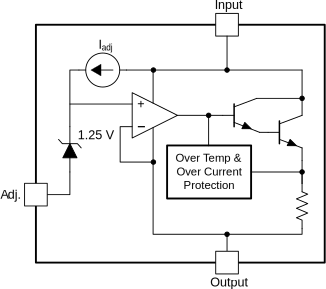
\includegraphics[height=5.9cm]{img/LM317.pdf}
					\caption{Blokové schéma LM317}
					\label{graf:1}
				\end{figure}
			\end{minipage}
		\end{tabular}
	\end{center}	
\end{table}

LM25085 je regulátor PFET tranzistorů učený do spínaných snižujících měničů s vysokou účinností (buck). Naproti tomu LM317 je notoricky známý integrovaný obvod určený především jako lineární stabilizátor napětí, popřípadě drobnou úpravou okolních součástek a zapojení jako zdroj stabilního proudu.
	\clearpage
\section{Výpočty hodnot součástek pro LM25085 PFET kontrolér}

\begin{table}[H]
	\begin{center}

		\begin{tabular}{c | c}
			\begin{minipage}{0.3\textwidth}
				\begin{eqnarray}
					V_{IN} &=& (18\div 32)~V \nonumber\\
					V_{\overline{IN}} &=& \dfrac{18 + 32}{2} = 25~V \nonumber\\\nonumber\\
					V_{OUT} &=& 9~V \nonumber\\
					I_{OUT} &=& I_{out_1} + I_{out_2} \nonumber\\
					I_{OUT} &=& 2,4 + 0,5 \doteq 3~A \nonumber\\ \nonumber\\
					F_{SW} &=& 300~kHz \nonumber\\
					V_{RIPPLE} &=& 5~mV_{pp} \nonumber					
				\end{eqnarray}
			\end{minipage}

	&		
				
			\begin{minipage}{0.7\textwidth}
				\begin{figure}[H]
					\begin{center}\resizebox{0.8\textwidth}{!}
					{
						\begin{circuitikz}
							%\draw[help lines, thick] (0,0) grid (15,15);	
							\draw (5,6) node[LM25085] (ic1) {\textbf{LM25085}};
							
							\draw (-2,9) to[eC=$C_{IN}$, *-*] (-2, 0);
							\draw (0,9) to[C=$C_{BYP}$, *-*] (0, 0);

							\draw (2,9) to[short] (2,12) to[short] (9,12) to[short] (9,7);							
							\draw (2,9) to[R=$R_T$, *-] (2,7) to[short] (3,7);
							
							\draw (7,9) to[short] (7.25,9) to[C=$C_{VCC}$, -*] (7.25, 12);
							
							\draw (7.25,7) to[short, *-] (7.25,7.8) to[C=$C_{ADJ}$, -*] (9,7.8);
							\draw (9,7) to[R=$R_{ADJ}$, *-] (7,7);
							
							\draw (9,7) to[R=$R_{SEN}$] (9,5);							
							\draw (9,7) to[R=$R_{SEN}$] (9,5);							
							\draw (9,4) node[pfet]{};
							\draw (9,0) to[sD-, *-] (9,2) to[short] (9,3.5);

														
							%\draw (9,3) to[short, *-] (10,3) to[short] (10,4) to[L=$L_1$] (12,4);
							\draw (9,3) -| (10,4) to[L=$L_1$] (12,4);
							\draw (9,3) to[short,*-] ++(0,0); 
							\draw (14,4) to[R=$R_{RFB2}$, *-*] (14,2) to[R=$R_{RFB1}$, -*] (14,0);
							\draw (12,4) to[C=$C_{FF}$, *-*] (12,2);

							
							\draw (16,4) to[eC=$C_{OUT}$, *-*] (16, 0);
							
													
							% ISEN
							\draw (7,5) to[short, -*] (9,5) to[short, -*] (9,4.27) to[short] (9,4);				
							% PGATE							
							\draw (7,4) to[short] (8.2,4);
							%FB
							\draw (7,3) to[short] (7.25,3) to[short] (7.25,2) to[short] (14,2);
							%GND
							\draw (3,3) to[short] (2,3) to[short, -*] (2,0);
							
							% svorky							
							\draw (-4,0) to[short, o-o] (18,0);
							\draw (-4,9) to[short, o-] (3,9);
							\draw (12,4) to[short, -o] (18,4);
							
							
							% napětí a proudy
							\draw (-4,9) to[open, v=$V_{IN}$] (-4,0);
							\draw (18,0) to[open, v<=$V_{OUT}$] (18,4);
							\draw (14,4) to[open, i=$I_{OUT}$] (18,4);
							
									

							

						\end{circuitikz}
					}
					\end{center}
					\caption{Snižující spínaný měnič}
				\end{figure}
			\end{minipage}
		\end{tabular}
	\end{center}	
\end{table}

\indent\indent Výpočet střídy spínání:
\begin{equation}
D = \dfrac{V_{OUT}}{V_{IN}} = \dfrac{t_{ON}}{t_{ON} + t_{OFF}} = t_{ON} \cdot F_S =
\left\lbrace
\begin{array}{ccl}
\dfrac{9}{18} & = & \underline{\underline{0,5}} \\\\
\dfrac{9}{25} & = & \underline{\underline{0,36}} \\\\
\dfrac{9}{32} & \doteq & \underline{\underline{0,28}}
\end{array}
\right.
\nonumber
\end{equation}

Výpočet doby otevření PFETu:
\begin{equation}
t_{ON} = \dfrac{D}{F_{S}} = \dfrac{V_{OUT}}{V_{IN} \cdot F_S} 
\left\lbrace
\begin{array}{ccl}
\dfrac{9}{18 \cdot 300 \cdot 10^{3}} & \doteq & \underline{\underline{1,667~\mu s}} \\\\
\dfrac{9}{25 \cdot 300 \cdot 10^{3}} & = & \underline{\underline{1,2~\mu s}} \\\\
\dfrac{9}{32 \cdot 300 \cdot 10^{3}} & = & \underline{\underline{937,5~ns}}
\end{array}
\right.
\nonumber
\end{equation}

Výpočet děliče zpětné vazby: $R_{FB1}$ zvolím $1~k\Omega$
\begin{equation}
R_{FB2} = \left( \dfrac{V_{OUT}}{1,25} - 1 \right) \cdot R_{FB1} = \left( \dfrac{9}{1,25} -1 \right) \cdot 10^{3} = \underline{\underline{6,2~k\Omega}}
\nonumber
\end{equation}


Výpočet výstupního napětí:
\begin{equation}
V_{OUT} = 1,25 \cdot \left( \dfrac{R_{FB1} + R_{FB2}}{R_{FB1}} \right) = 1,25 \cdot \left(1 + \dfrac{R_{FB2}}{R_{FB1}} \right) = 1,25 \cdot \left( 1+ \dfrac{6,2}{1} \right) = \underline{\underline{9~V}}
\nonumber
\end{equation}

Výpočet kondenzátoru zpětné vazby:
\begin{equation}
C_{FF} = \dfrac{3 \cdot T_{on_{(max)}}}{\dfrac{R_{BF1} \cdot R_{BF2}}{R_{BF1} + R_{BF2}}} =
 \dfrac{3 \cdot 1,667 \cdot 10^{-6}}{\dfrac{1 \cdot 10^{3} \cdot 6,2 \cdot 10^{3}}{1 \cdot 10^{3} + 6,2 \cdot 10^{3}}} = 5,8~nF \doteq \underline{\underline{6,8~nF}}
\nonumber
\end{equation}

Velikost rezistoru $R_T$ nastavuje spínací frekvenci: $R_T$ je v $k\Omega$
\begin{eqnarray}
R_T &=& \dfrac{V_{OUT} \cdot (V_{IN} - 1,56)}{1,45 \cdot 10^{-7} \cdot V_{IN} \cdot F_S} - \dfrac{t_D \cdot (V_{IN} - 1,56)}{1,45 \cdot 10^{-7}} - 1,4 \nonumber\\
R_T &=& \dfrac{9 \cdot (25 - 1,56)}{1,45 \cdot 10^{-7} \cdot 25 \cdot 300 \cdot 10^{3}} - \dfrac{t_D \cdot (25 - 1,56)}{1,45 \cdot 10^{-7}} - 1,4 = 193,016~k\Omega \doteq \underline{\underline{180~k\Omega}}
\nonumber
\end{eqnarray}


Výpočet vyhlazovací cívky:
\begin{equation}
L_1 = \dfrac{t_{ON_{(min)}} \cdot \left(V_{IN_{(max)}} - V_{OUT} \right)}{0,2 \cdot I_{OUT}} = \dfrac{937,5 \cdot 10^{-9} \cdot (32 - 9)}{0,2 \cdot 3} \doteq \underline{\underline{36~\mu H}}
\nonumber
\end{equation}
Vzhledem k toleranci nominální hodnoty vyráběných cívek zvolím cívku $\underline{\underline{47~\mu H}}$ abych měl rezervu, pokud bude hodnota cívka v dolní části tolerančního pásma.
\\\\\indent
Výpočet vyhlazovacího kondenzátoru:
\begin{equation}
C_{OUT} = \dfrac{0,2 \cdot I_{OUT}}{8 \cdot F_S \cdot V_{RIPPLE}} = \dfrac{0,2 \cdot 3}{8 \cdot 300 \cdot 10^{3} \cdot 5 \cdot 10^{-3}} = 50~\mu F \doteq \underline{\underline{68~\mu F}}
\nonumber
\end{equation}

Vzhledem k tomu, že tento kondenzátor je na výstupu spínaného měniče kde se výstupní napětí pohybuje okolo $9~V$, tak tento kondenzátor by měl být dimenzován minimálně na $16~V$ pro jistotu na $20~V$.
\\\\\indent
Výpočet vstupního kondenzátoru:
\begin{equation}
C_{IN} + C_{BYP} = \dfrac{I_{OUT} \cdot t_{ON_{(max)}}}{\Delta V} = \dfrac{3 \cdot 1,667 \cdot 10^{-6}}{0,5} \doteq \underline{\underline{10~\mu F}}
\nonumber
\end{equation}

$C_{BYP}$ zvolím podle doporučení datasheetu jako $1~\mu F$ a $C_{IN}$ zvolím jako $10~\mu F$ na $50~V$, protože vstupní napětí může být až $32~V$.
\\\\\indent
Výpočet zvlnění proudu:
\begin{equation}
\Delta I = \dfrac{t_{ON_{(min)}} \cdot \left(V_{IN_{(max)}} - V_{OUT} \right)}{L_1} = \dfrac{937,5 \cdot 10^{-9} \cdot (32 - 9)}{47 \cdot 10^{-6}} \doteq \underline{\underline{459~mA}}
\nonumber
\end{equation}

Velikost minimální hodnoty proudové limitace:
\begin{equation}
I_{CL_{(min)}} = I_{OUT} + \dfrac{\Delta I}{2} = 3 + \dfrac{0,459}{2} \doteq \underline{\underline{3,25~A}}
\nonumber
\end{equation}

Výpočet minimálního proudového limitu se započítanou chybou offsetu komparátoru:
\begin{equation}
I_{CL_{(min)_{offset}}} = I_{CL_{(min)}} + \dfrac{9 \cdot 10^{-3}}{R_{SEN}} = 3,25 + \dfrac{9 \cdot 10^{-3}}{10 \cdot 10^{-3}} = \underline{\underline{4,15~A}}
\nonumber
\end{equation}

Výpočet rezistoru $R_{ADJ}$:
\begin{equation}
R_{ADJ} = \dfrac{I_{CL_{(min)_{offset}}} \cdot R_{SEN}}{I_{ADJ_{(min)}}} = \dfrac{4,15 \cdot 10 \cdot 10^{-3}}{32 \cdot 10^{-6}} = 1297~\Omega \doteq \underline{\underline{1,5~k\Omega}}
\nonumber
\end{equation}

$C_{ADJ} = 1~nF$ hodnota podle doporučení v datasheetu, filtruje šum s ADJ pinu, zabraňuje nechtěnému sepnutí komparátoru.
\\\\
\indent Velikost rezistoru $R_{SEN}$ výrobce doporučuje $10~m\Omega$, výkonová ztráta na rezistoru je:
\begin{equation}
P_{R_{SEN}} = I_{CL_{(min)}}^2 \cdot R_{SEN} = 3,25^2 \cdot 10 \cdot 10^{-3} \doteq \underline{\underline{106~mW}}
\nonumber
\end{equation}
Podle toho je důležité zvolit pouzdro, které snese takovéto zatížení. Vypočítané zatížení by snesl rezistor v pouzdru 0805, který vydrží $125~mW$ či pouzdro 1206 které vydrží do $250~mW$, pro jistotu, ale volím pouzdro 1210, které vydrží výkon až $500~mW$ tím zajistím že součástka nebude na pokraji svých možností a bude mít dostatečnou životnost.
\\\\
Hodnota kondenzátoru $C_{VCC}$ je dle doporučení datasheetu $470~nF$.
	\clearpage
\section{Výpočty hodnot součástek pro lineární stabilizátor s LM317}

\begin{table}[H]
	\begin{center}

		\begin{tabular}{c | c}
			\begin{minipage}{0.2\textwidth}
				\begin{eqnarray}
					V_{i} &=& 9~V \nonumber\\
					V_o &=& 4,5~V \nonumber\\
					I_o &=& 0,5~A \nonumber\\\nonumber\\
					V_{REF} &=& 1,25~V \nonumber\\
					I_{ADJ} &=& 50~\mu A \nonumber
				\end{eqnarray}
			\end{minipage}

	&		
				
			\begin{minipage}{0.6\textwidth}
				\begin{figure}[H]
					\begin{center}
						\begin{circuitikz}
							%\draw[help lines, thick] (0,0) grid (10,8);	
							\draw (3,4) node[ic3pin] (ic1) {\textbf{LM317}};
							
							
							%(0,0) node[anchor=east] {Vstup}			
							\draw (0,0) to[short, o-o] (10,0);
							\draw (0,4) to[short, o-] (2,4);
							\draw (4,4) to[short, -o] (10,4);
							
							\draw (3,3) to[short, -, i=$I_{ADJ}$] (3,2) to[short] (7,2);
							
							\draw (5.5,4) to[R, R=$R_1$, *-*, v=$V_{REF}$] (5.5,2) to[R, R=$R_2$, -*] (5.5,0);
							\draw (7,2) to[C=$C_{ADJ}$, -*] (7,0);								
							
							\draw (7,2)
							to[D-=$D_1$, *-*] (7,4)
							to[short, -] (7,6)
							to[D-=$D_1$] (1,6)
							to[short] (1,4);							
							
							
							\draw (1,4) to[C=$C_I$, *-*] (1,0);							
							\draw (9,4) to[C=$C_O$, *-*] (9,0);
							
							\draw (0,4) to[open, v=$V_i$] (0,0);
							\draw (10,0) to[open, v<=$V_o$] (10,4);
							
							\draw (7,4) to[open, -o, i=$I_o$] (10,4);
							
							%\draw (2,0) node[ground] {};					

							

						\end{circuitikz}
					\end{center}
					\caption{Lineární stabilizátor}
				\end{figure}
			\end{minipage}
		\end{tabular}
	\end{center}	
\end{table}


\indent\indent Výpočet zpětnovazebního děliče:
\begin{equation}
R_2 = \dfrac{V_o - V_{REF}}{\dfrac{V_{REF}}{R_1} + I_{ADJ}} = \dfrac{4,5 - 1,25}{\dfrac{1,25}{R_1} + 50 \cdot 10^{-6}}
\nonumber
\end{equation}

K výpočtu nejpřesnější kombinace rezistorů $R_1$ a $R_2$ jsem napsal skript LM317.py, který vypočítá pro řady $E3 \div E192$ nejvhodnější kombinace rezistorů. Výsledek skriptu pro $V_o = 4,5~V$ je uveden v tabulce.

\begin{table}[H]
	\caption{Hodnoty zpětnovazebného děliče pro LM317}	
	\begin{center}				
		\newcolumntype{R}{>{\raggedleft\arraybackslash}X}
		\newcolumntype{L}{>{\raggedleft\arraybackslash}X}
		\newcolumntype{C}{>{\centering\arraybackslash}X}		
		\begin{tabularx}{0.8\textwidth}{!\vcara C|C|C|C !\vcara}
			\hcara 
			\textbf{řada} & $\mathbold{R_1~[\Omega]}$ & $\mathbold{R_2~[\Omega]}$ & $\mathbold{V_o~[V]}$ \\\hcara 
			E3 & 100 & 220 & 4,0110 \\\hline 
			E6 & 680 & 1500 & 4,0824 \\\hline 
			E12 & 470 & 1200 & 4,5015 \\\hline 
			E24 & 510 & 1300 & 4,5013 \\\hline 
			E48 & 953 & 2370 & 4,4771 \\\hline 
			E96 & 562 & 1430 & 4,5021 \\\hline 
			E192 & 229 & 590 & 4,5000 \\\hcara
		\end{tabularx} 
	\end{center}
\end{table}

Výpočet výstupního napětí:
\begin{equation}
V_o = V_{REF} \cdot \left(1 + \dfrac{R_2}{R_1} \right) + I_{ADJ} \cdot R_2 = 1,25 \cdot \left(1 + \dfrac{590}{229} \right) + 50 \cdot 10^{-6} \cdot 590 \doteq \underline{\underline{4,5~V}}
\nonumber
\end{equation}

Vstupní a výstupní kondenzátor mají hodnotu podle doporučení datasheetu a to: $C_i = 100~nF$ a $C_o = 1~\mu F$. Na $C_o$ je možné ještě paralelně přiletovat $C_{BYPASS}$ v pouzdru 0805 pro přemostění vysokofrekvenčního rušení. Kondenzátor pro stabilizaci napěťové reference má také hodnotu dle doporučení výrobce $C_{ADJ} = 10~\mu F$.


		

	\clearpage
\section{Výpočty chlazení a výkonových ztrát}

\indent\indent Výpočet výkonové ztráty na LM317:
\begin{equation}
P_{LM317} = (V_i - V_o) \cdot I_o = (9 - 4,5) \cdot 0,5 = \underline{\underline{2,25~W}}
\nonumber
\end{equation}

Výpočet výkonové ztráty na schottkyho diodě:
\begin{equation}
P_{D} = V_F \cdot I_{OUT} \cdot \left(1-D_{(min)} \right) = 3 \cdot 0,455 \cdot (1-0,28) \doteq \underline{\underline{962~mW}}
\nonumber
\end{equation}

Výpočet výkonové ztráty na PFETu:
\begin{equation}
P_{PFET} = V_{IN_{(max)}} \cdot \left( Q_G \cdot F_S + I_{IN}\right) = 32 \cdot (24 \cdot 10^{-9} \cdot 300 \cdot 10^{3} + 1,3 \cdot 10^{-3}) = \underline{\underline{272~mW}}
\nonumber
\end{equation}

Výpočet celkového tepelného odporu chlazení LM317:
\begin{equation}
R_{thsys_{(LM317)}} = \dfrac{\vartheta_{j_{(max)}} - \vartheta_a}{P_{LM317}} = \dfrac{150 - 80}{2,25} \doteq \underline{\underline{32~KW^{-1}}}
\nonumber
\end{equation}

Výpočet celkového tepelného odporu chlazení schottkyho diody:
\begin{equation}
R_{thsys_{(D)}} = \dfrac{\vartheta_{j_{(max)}} - \vartheta_a}{P_{D}} = \dfrac{150 - 80}{0,962} \doteq \underline{\underline{73~KW^{-1}}}
\nonumber
\end{equation}

Výpočet celkového tepelného odporu chlazení PFETu:
\begin{equation}
R_{thsys_{(PFET)}} = \dfrac{\vartheta_{j_{(max)}} - \vartheta_a}{P_{PFET}} = \dfrac{175 - 80}{0,272} \doteq \underline{\underline{345~KW^{-1}}}
\nonumber
\end{equation}


\begin{figure}[H]
  \centering
  \includegraphics{img/DPS_odpor.pdf}
  \caption{Graf závislosti tepelného odporu plošného spoje na jeho ploše}
  \label{graf:1}
\end{figure}

Z grafů vyplývá, že shottkyho diodu a PFET nebude problém uchladit plošným spojem, pro LM317 ale vychází plocha mědi na můj vkus příliš veliká cca $7~cm \cdot 7~cm$ a tak zvolím klasické chlazení hliníkovým profilem. Vybral jsem chladič s tepelným odporem $11~KW^{-1}$, takže teplota křemíkového čipu LM317 by měla být nižší, než teplota maximální na kterou jsem počítal celkový tepelný odpor.
	\clearpage
\section{Realizace napájecího zdroje}


\begin{figure}[H]
	\centering 	
	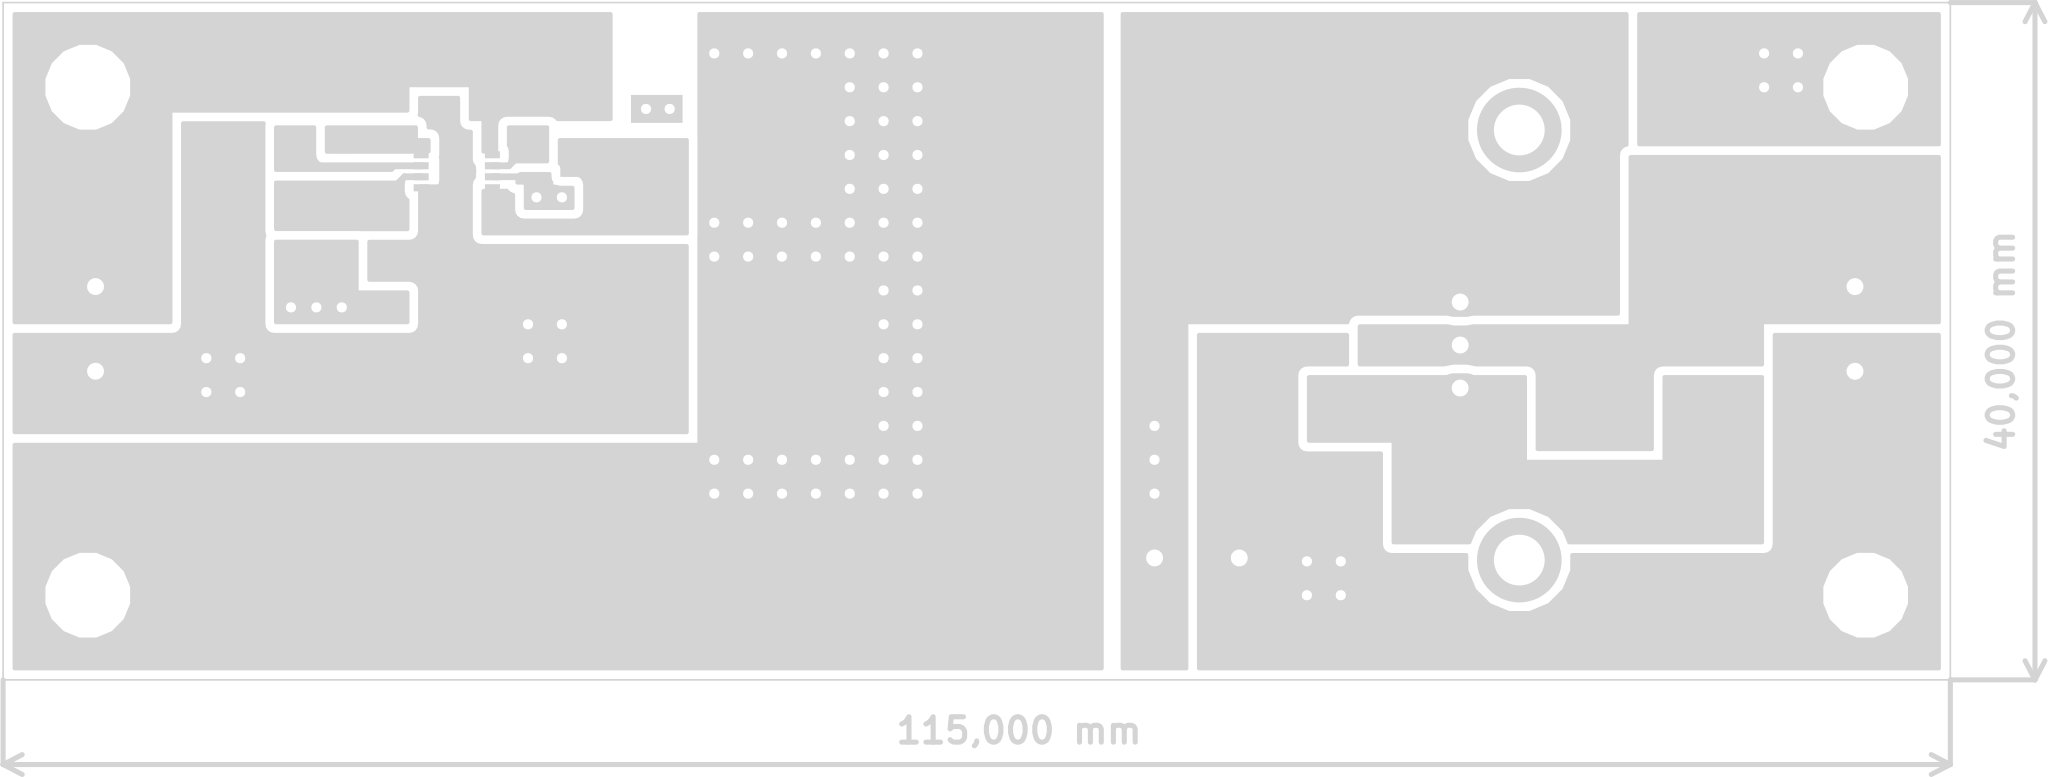
\includegraphics[width=17cm]{../design/PDF_out/top.pdf}
	\caption{Plošný spoj vrstva součástek}	
\end{figure}

\begin{figure}[H]
	\centering 	
	\includegraphics[width=17cm]{../design/PDF_out/bot.pdf}
	\caption{Plošný spoj vrstva mědi}	
\end{figure}

\begin{figure}[H]
	\centering 	
	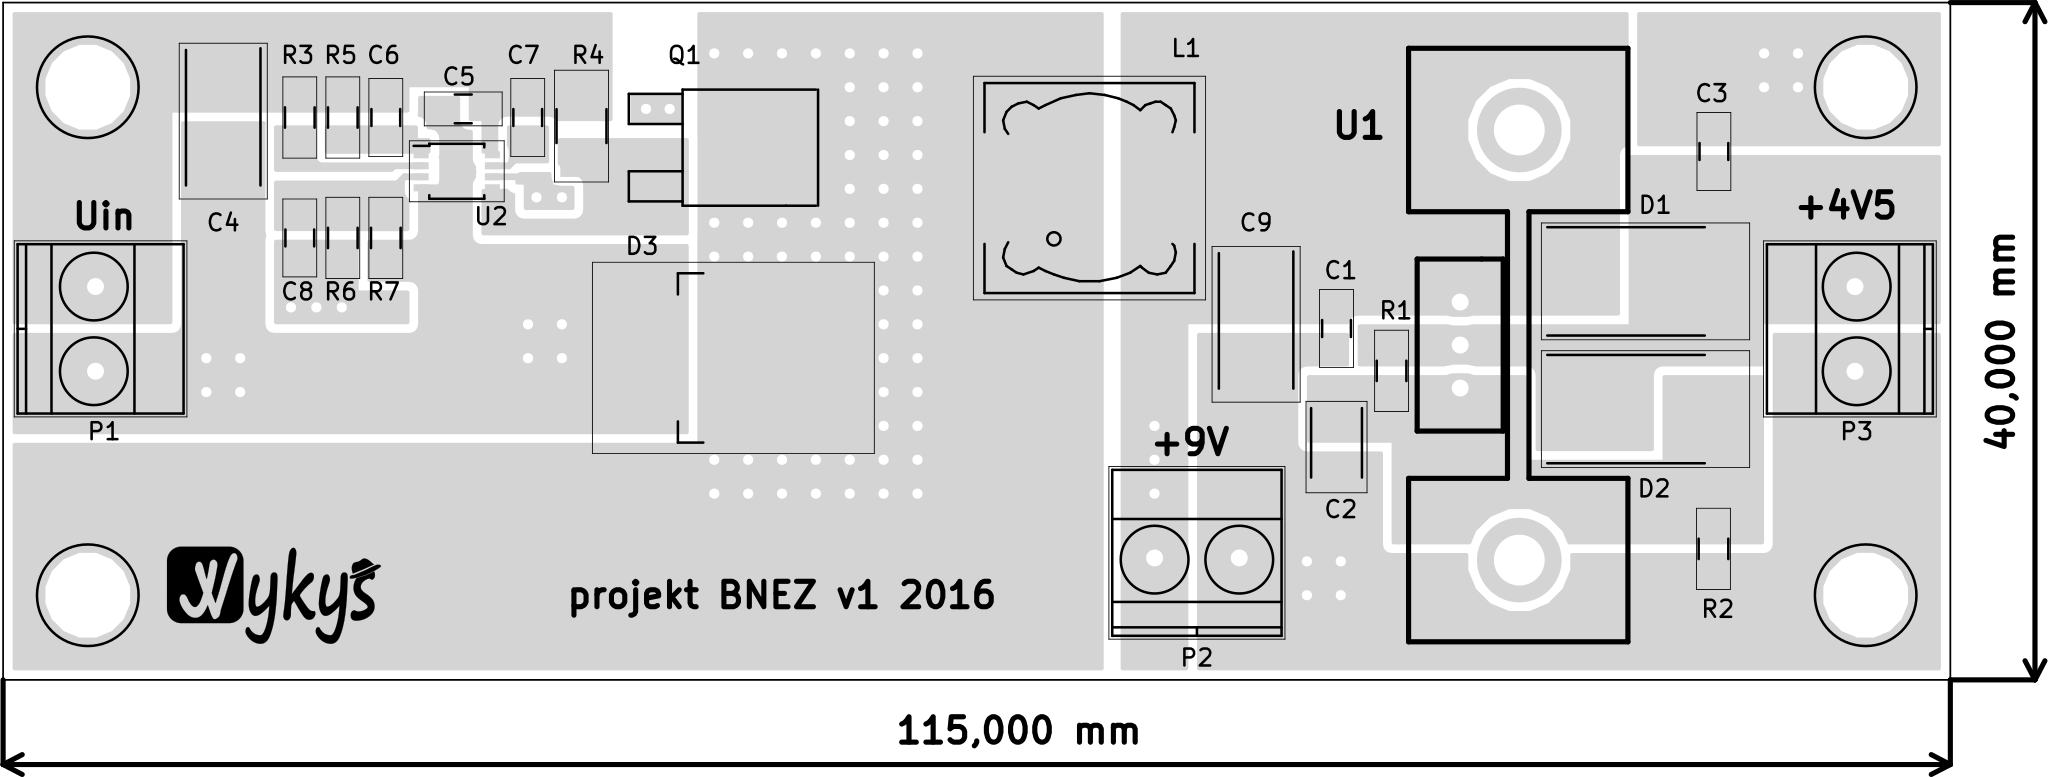
\includegraphics[width=17cm]{../design/PDF_out/osazovak.pdf}
	\caption{Osazovací výkres}	
\end{figure}




\begin{figure}[H]
	\centering 	
	\includegraphics[width=17cm]{../design/PDF_out/prokov.pdf}
	\caption{Vrtací plán prokovené díry}	
\end{figure}

\begin{figure}[H]
	\centering 	
	\includegraphics[width=17cm]{../design/PDF_out/prokov_ne.pdf}
	\caption{Vrtací plán neprokovené díry}	
\end{figure}

\begin{table}[H]
	\caption{BOM rozpiska materiálu}
	\begin{figure}[H]
		\centering 	
		\includegraphics[width=17cm]{../BOM.pdf}
	\end{figure}
\end{table}	





\newgeometry{left=1.25cm,bottom=1cm, top=2cm}
\begin{landscape}	
	\begin{figure}[h]
		\centering 	
		\includegraphics[height=\textwidth]{../design/xvykyd06_zdroj.pdf}
		\caption{Schéma zapojení napájecího zdroje}	
	\end{figure}
\end{landscape}
\restoregeometry


\begin{figure}[H]
	\centering 	
	\includegraphics[width=\textwidth]{../design/img/xvykyd06_zdroj_6.png}
	\caption{Plošný pohled na stranu součástek bez součástek}	
\end{figure}



\begin{figure}[H]
	\centering 	
	\includegraphics[width=\textwidth]{../design/img/xvykyd06_zdroj_2.png}
	\caption{Plošný spoj pohled na stranu součástek}	
\end{figure}

\begin{figure}[H]
	\centering 	
	\includegraphics[width=\textwidth]{../design/img/xvykyd06_zdroj_5.png}
	\caption{Plošný spoj pohled na stranu spojů}	
\end{figure}

\begin{figure}[H]
	\centering 	
	\includegraphics[width=\textwidth]{../design/img/xvykyd06_zdroj_3.png}
	\caption{Napájecí zdroj pohled ze strany}	
\end{figure}

\begin{figure}[H]
	\centering 	
	\includegraphics[width=\textwidth]{../design/img/xvykyd06_zdroj_4.png}
	\caption{Napájecí zdroj pohled zepředu}	
\end{figure}

\begin{figure}[H]
	\centering 	
	\includegraphics[width=\textwidth]{../design/img/xvykyd06_zdroj_1.png}
	\caption{Napájecí zdroj pohled zezadu}	
\end{figure}





Gerber soubory jsou generovány na POOL servis gatema.
 
	\label{konec}
\end{document}
